%!TEX program = xelatex

\documentclass[12pt]{beamer}
\usepackage{graphicx}

\setlength{\parindent}{0pt}

%\setbeameroption{show notes}
\makeatletter
\def\beamer@framenotesbegin{% at beginning of slide
    \gdef\beamer@noteitems{}%
    \gdef\beamer@notes{{}}% used to be totally empty.
}
\makeatother

% Theme stuff
% -----------
\usetheme{default}
\beamertemplatenavigationsymbolsempty
%\setbeamertemplate{itemize item}[circle]
\setbeamertemplate{itemize items}{$\bullet$}
\setbeamertemplate{itemize subitem}{$\circ$}
\setbeamercolor{itemize item}{fg=black}
\setbeamercolor{itemize subitem}{fg=black}
\setbeamercolor{itemize subsubitem}{fg=black}
\setbeamertemplate{enumerate items}[default]
\setbeamercolor{enumerate item}{fg=black}
\setbeamercolor{enumerate subitem}{fg=black}
%\setbeamertemplate{footline}[frame number]

% Algorithm stuff
% ---------------
\usepackage[vlined,linesnumbered]{algorithm2e}
\newcommand\mycommfont[1]{\textcolor{gray}{#1}}
\SetCommentSty{mycommfont}

% Font stuff
% ----------
\usepackage[no-math]{fontspec}
\defaultfontfeatures{Mapping=tex-text}
\setsansfont[BoldFont=P22UndergroundBook,
			 SmallCapsFont=P22UndergroundLightSC]{P22UndergroundLight}
\setmonofont{Hack}

% bib stuff
\setbeamertemplate{bibliography item}{[\theenumiv]}

% full frame picture
\newcommand{\fullframepicture}[1]{
%\mode
{
\usebackgroundtemplate{\includegraphics[width=\paperwidth]{#1}}
\begin{frame}[plain]
\end{frame}
}
\mode{\usebackgroundtemplate{}}
%\mode*
}


% Define colors
% -------------
\usepackage{xcolor}
\definecolor{BGDarkGrey}{RGB}{50,50,50}
\definecolor{BGBlue}{RGB}{77,143,249}
\definecolor{LightGrey}{RGB}{200,200,200}
\definecolor{Grey50}{RGB}{128,128,128}
\definecolor{LBlue}{HTML}{29B6F6}
\definecolor{Blue}{HTML}{42A5F5}
\definecolor{Orange}{HTML}{FFA726}
\definecolor{LGreen}{HTML}{9CCC65}
\definecolor{Green}{HTML}{66BB6A}
\definecolor{Red}{HTML}{EF5350}
\definecolor{Amber}{HTML}{FFCA28}
\definecolor{Yellow}{HTML}{FFEE58}
\definecolor{Cyan}{HTML}{26C6DA}
\definecolor{Indigo}{HTML}{5C6BC0}
\definecolor{Lime}{HTML}{D4E157}
\definecolor{BlueGrey}{HTML}{78909C}
\definecolor{DeepOrange}{HTML}{FF7043}
\definecolor{Grey}{HTML}{424242}
\definecolor{Teal}{HTML}{26A69A}
\definecolor{PaleYellow}{RGB}{255,255,153}

\definecolor{DhakaBlue}{RGB}{102,167,221}
\definecolor{WikiGrey}{RGB}{252,252,252}

\renewcommand{\arraystretch}{2}

% Table package
% -------------
\usepackage{booktabs}

% Background
% ----------
\usepackage{tikz}

\begin{document}


% Title
\setbeamercolor{normal text}{fg=Grey, bg=white}
\usebeamercolor[fg]{normal text}
\begin{frame}

	\null
	\vfill
	%\centering
	\textcolor{black}{\textsc{\large A Comparative Study of Techniques for Estimation and Inference of Nonlinear Stochastic Time Series}} \\
	\vspace{1.5\baselineskip}
	\noindent\textcolor{black}{\rule{\textwidth}{0.4pt}} \\
	\vspace{2\baselineskip}
	Dexter Barrows, B.Sc. \\
	\vspace{1\baselineskip}
	Masters Thesis Defence \\
	McMaster University \\
	April 2016
	\vfill

\end{frame}


% Authors
\setbeamercolor{normal text}{fg=Grey, bg=white}
\usebeamercolor[fg]{normal text}
\begin{frame}

	\vspace{\baselineskip}
	\begin{columns}
		\begin{column}{0.8\textwidth}
			{\large
			\begin{enumerate}
				\item Framing
				\item Stochastic SIR Model
				\item Hamiltonian HMC
				\item Iterated Filtering 2
				\item Fitting Results
				\item Forecasting Frameworks
				\item S-maps \& Seasonal Outbreaks
				\item Spatiotemporal Epidemics
				\item Parallelism \& Future Directions
			\end{enumerate}
			}
		\end{column}
	\end{columns}

\end{frame}

%% 1. INTRODUCTION
%% --------------------------------------------------------------------------------------
%% --------------------------------------------------------------------------------------

% Section title
\setbeamercolor{normal text}{fg=white, bg=BGBlue}
\usebeamercolor[fg]{normal text}
\begin{frame}

	\vspace{2cm}
	\hspace{2.5cm} {\Huge Framing }
	\begin{tikzpicture}[overlay]
	    \node[at=(current page.center), shift={(-4.5 cm, -4.7 cm)}, opacity=0.25] {
	    	\fontsize{200pt}{0pt}\selectfont
	        \color{white}{1}
	    };
	\end{tikzpicture}

\end{frame}

\setbeamercolor{normal text}{fg=Grey, bg=white}
\usebeamercolor[fg]{normal text}
\hspace{-1.55cm}
\begin{frame}[plain]

	\hspace{-2cm}
	
\includegraphics[width=\paperwidth,keepaspectratio=true]{images/wordcloud-6}

\end{frame}


%% 2. Stochastic SIR model
%% --------------------------------------------------------------------------------------
%% --------------------------------------------------------------------------------------

% Section title
\setbeamercolor{normal text}{fg=white, bg=Amber}
\usebeamercolor[fg]{normal text}
\begin{frame}

	\vspace{2cm}
	\hspace{0cm} {\Huge Stochastic SIR Model } \\
	\begin{tikzpicture}[overlay]
	    \node[at=(current page.center), shift={(3.2 cm, -4 cm)}, opacity=0.25] {
	    	\fontsize{200pt}{0pt}\selectfont
	        \color{white}{2}
	    };
	\end{tikzpicture}

\end{frame}

% Basic Stochastic SIR
\setbeamercolor{normal text}{fg=white, bg=Grey}
\setbeamercolor{footline}{parent=normal text}
\usebeamercolor[fg]{normal text}
\begin{frame}

	\null
	{\large \textcolor{Cyan}{Stochastic SIR model}}
	\vfill

	\centering
	\begin{align*}
		\dfrac{dS}{dt} 	& = - \beta S I \\
		\dfrac{dI}{dt} 	& = \beta S I - \gamma I \\
		\dfrac{dR}{dt} 	& =  \gamma I
	\end{align*}
	\vspace{0.5\baselineskip}
	{\Large $+$}	\\
	\vspace{1\baselineskip}
	$\beta_{t+1} = \exp \left[ \beta_t + \eta \left( \bar{\beta} - \beta_t \right) + \mathcal{N}(0, \sigma_{\small\text{proc}}) \right]$

\end{frame}

\setbeamercolor{normal text}{fg=Grey, bg=white}
\usebeamercolor[fg]{normal text}
\begin{frame}

	\null
	\large
	Model simulations \\
	\vspace{\baselineskip}
	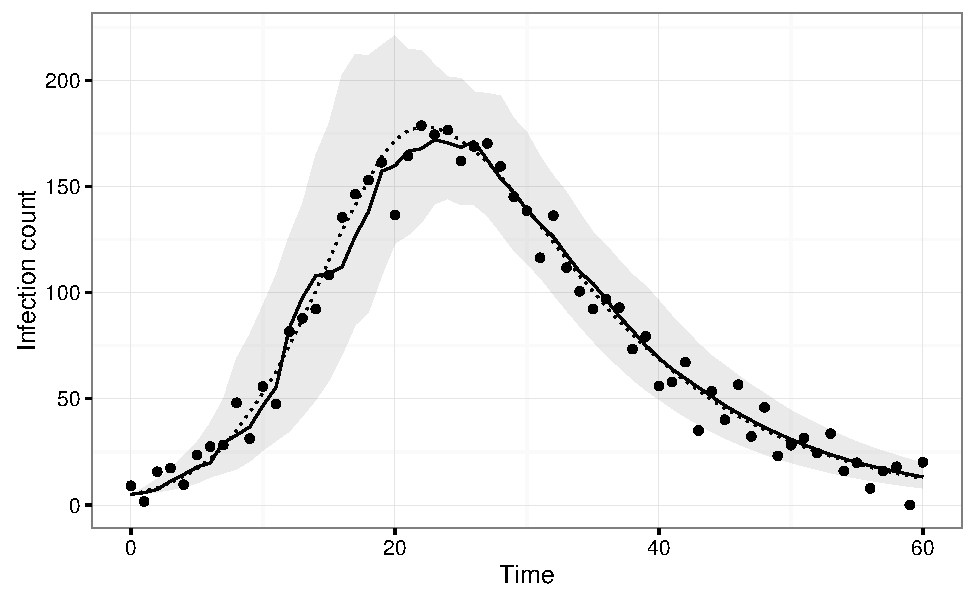
\includegraphics[width=\textwidth,height=\textheight,keepaspectratio=true]{../../writing/SC1/images/sirmean}
	
	\vspace{0.5\baselineskip}
	\tiny
	\centering
	Solid -- sample trajectory $\quad\cdot\quad$ dots -- sample data $\quad\cdot\quad$ dotted -- average $\quad\cdot\quad$ ribbon -- overall

\end{frame}


%% 3. HMC
%% --------------------------------------------------------------------------------------
%% --------------------------------------------------------------------------------------

% Section title
\setbeamercolor{normal text}{fg=white, bg=Green}
\usebeamercolor[fg]{normal text}
\begin{frame}

	\vspace{2cm}
	\hspace{0cm} {\Huge Hamiltonian MCMC }
	\begin{tikzpicture}[overlay]
	    \node[at=(current page.center), shift={(-5.2 cm, -4.7 cm)}, opacity=0.25] {
	    	\fontsize{200pt}{0pt}\selectfont
	        \color{white}{3}
	    };
	\end{tikzpicture}

\end{frame}


\setbeamercolor{normal text}{fg=Grey, bg=white}
\usebeamercolor[fg]{normal text}
\begin{frame}

	\begin{columns}
		\begin{column}[t]{0.5\textwidth}

			\large
			MCMC
			\vspace{1.5\baselineskip}

			\normalsize
			Iteratively construct Markov chain to approximate posterior

			\vspace{0.5\baselineskip}

			\footnotesize
			\begin{enumerate}
				\item Choose starting parameter set
				\item Generate N samples by
				\begin{enumerate}
					\footnotesize
					\item Propose new sample
					\item Compute acceptance ratio
					\item Accept/reject sample
				\end{enumerate}
			\end{enumerate}

			
		\end{column}
		\begin{column}[t]{0.5\textwidth}

			\large
			HMC
			\vspace{1.5\baselineskip}

			\normalsize
			Proposal via Hamiltonian dynamics

			\vspace{1.5\baselineskip}

			\footnotesize
			\begin{enumerate}
				\item Choose starting parameter set
				\item Generate N samples by
				\begin{enumerate}
					\footnotesize
					\item Resample moments
					\item Simulate Hamiltonian dynamics using Leapfrog integration
					\item Compute acceptance ratio
					\item Accept/reject sample
				\end{enumerate}
			\end{enumerate}


		\end{column}
	\end{columns}

\end{frame}


\setbeamercolor{normal text}{fg=Grey, bg=white}
\usebeamercolor[fg]{normal text}
\begin{frame}
	
	\null
	{\large Hamiltonian Dynamics}
	\vspace{\baselineskip}
	\vfill

	\footnotesize

	\begin{align*}
		& \text{Energy} & & \\
		& \quad\quad \text{Kinetic} 	& K(r) 					& = \frac{1}{2} r^T M^{-1} r \\
		& \quad\quad \text{Potential} 	& U(\theta) 			& = - \log(\mathcal{L}(\theta)p(\theta)) \\
		& & & \\
		& \text{Hamiltonian} 			& H(\theta,r)  			& = U(\theta) + K(r) \\
		& & & \\
		& \text{Dynamics simulation}	& \frac{d\theta}{dt} 	& = M^{-1} r \\
		& 								& \frac{dr}{dt}			& = - \nabla U (\theta) \\
	\end{align*}

	\vfill

\end{frame}


%% 4. IF2
%% --------------------------------------------------------------------------------------
%% --------------------------------------------------------------------------------------

% Section title
\setbeamercolor{normal text}{fg=white, bg=LBlue}
\usebeamercolor[fg]{normal text}
\begin{frame}

	\vspace{2cm}
	\hspace{0cm} {\Huge Iterated Filtering 2 }
	\begin{tikzpicture}[overlay]
	    \node[at=(current page.center), shift={(-4.7 cm, -4.7 cm)}, opacity=0.25] {
	    	\fontsize{200pt}{0pt}\selectfont
	        \color{white}{4}
	    };
	\end{tikzpicture}

\end{frame}

\setbeamercolor{normal text}{fg=Grey, bg=white}
\usebeamercolor[fg]{normal text}
\begin{frame}

	\null
	\hspace{-0.475cm}
	\large
	Basic particle filter
	\vspace{\baselineskip}

	\begin{columns}
		\begin{column}{0.45\textwidth}

			\footnotesize
			Iterative prediction-update cycle prunes particle cohort of poor parameter estimates

			\begin{enumerate}
				\item Initialize particles with parameter sets
				\item For each data point
				\begin{enumerate}
					\footnotesize
					\item Evolve particle states
					\item Weight via likelihood
					\item Resample proportional to weights
				\end{enumerate}
			\end{enumerate}
			
			
		\end{column}
		\begin{column}{0.55\textwidth}

			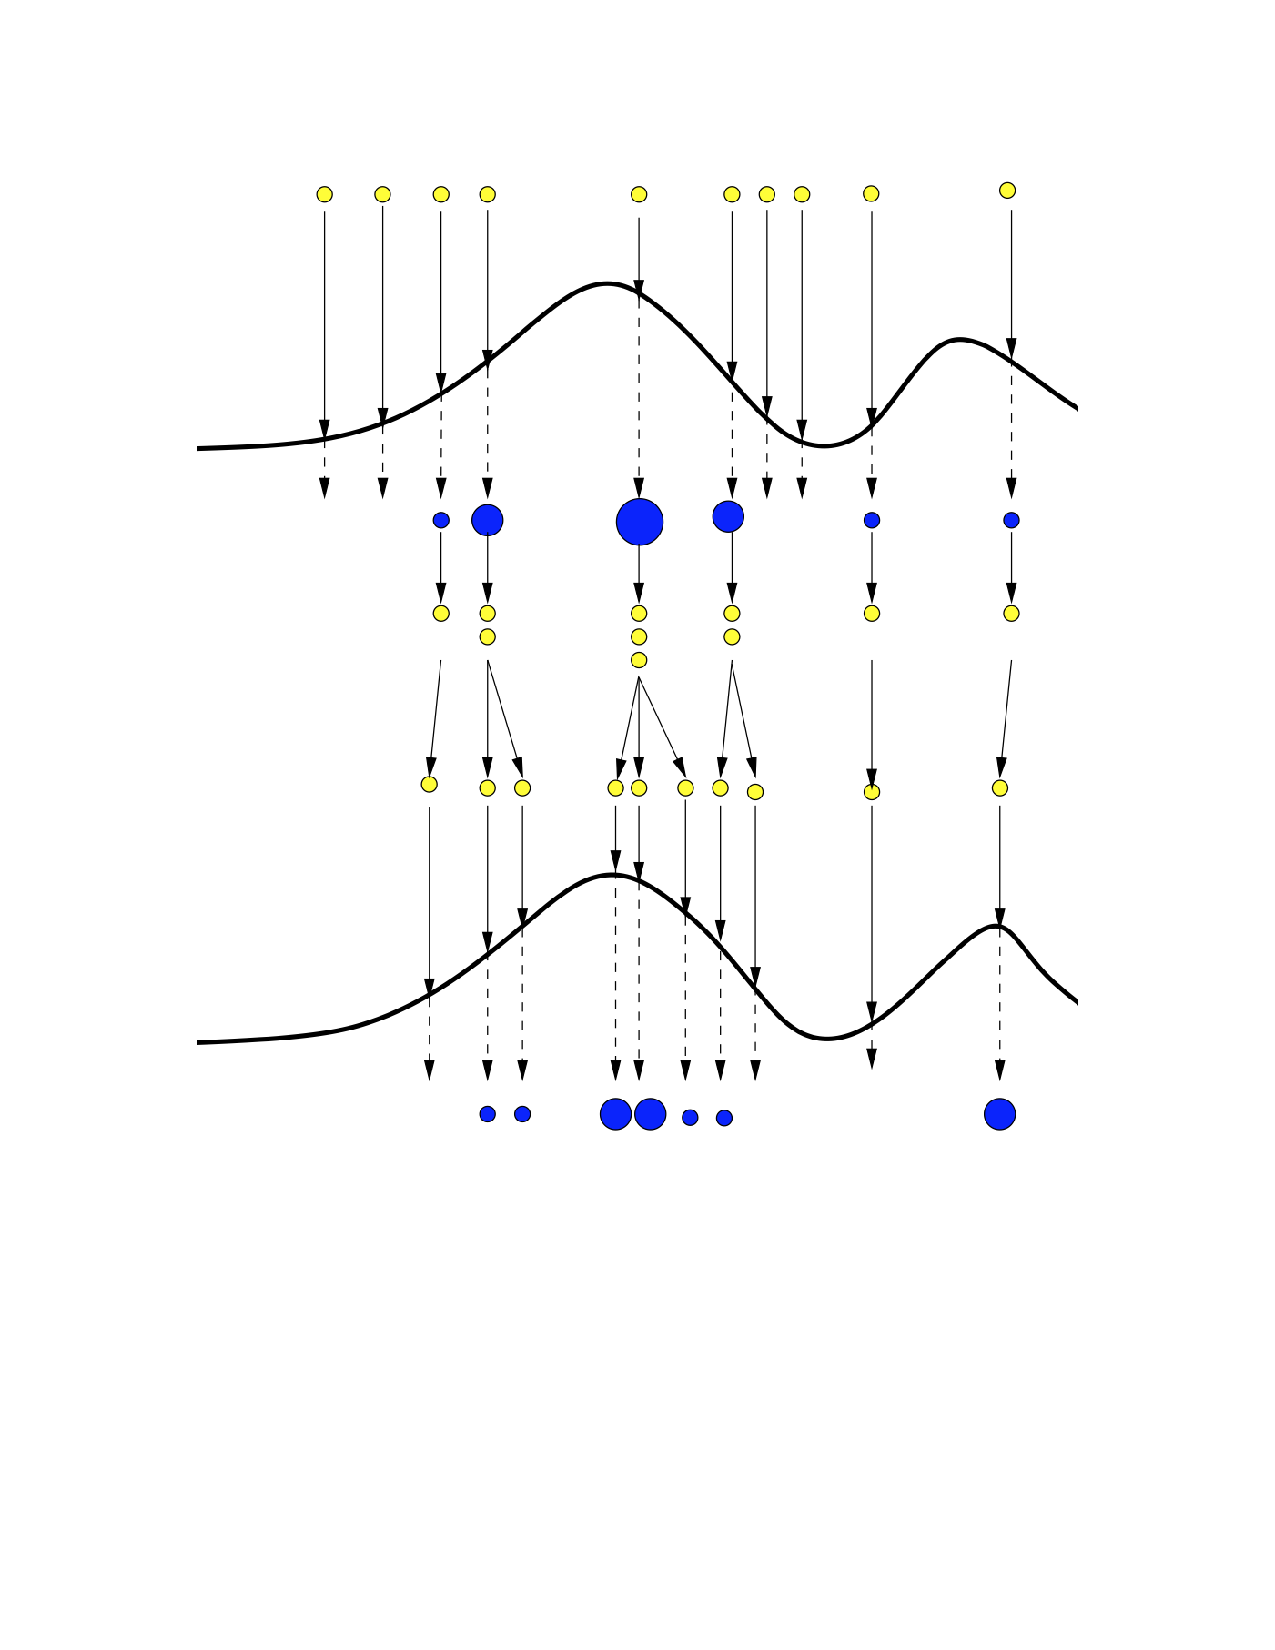
\includegraphics[width=\textwidth,height=0.9\textheight,keepaspectratio=true]{images/PF-diagram}

		\end{column}
	\end{columns}

	\centering
	\tiny
	Image source \cite{Doucet2001}

\end{frame}

\setbeamercolor{normal text}{fg=Grey, bg=white}
\usebeamercolor[fg]{normal text}
\begin{frame}

	\null
	\hspace{-0.475cm}
	\large
	Iterated Filtering 2 (IF2)
	\vspace{0.5\baselineskip}

	\begin{columns}
		\begin{column}[t]{0.5\textwidth}

			\footnotesize
			Evolution of MIF (IF1) \\
			\vspace{\baselineskip}
			Multiple passes through data \\
			\vspace{\baselineskip}
			Treat parameter estimates as stochastic processes
			\begin{itemize}
				\footnotesize
				\item Alleviates risk of particle collapse
				\item Process noise decreases with passes
			\end{itemize}

			
		\end{column}
		\begin{column}[t]{0.5\textwidth}

			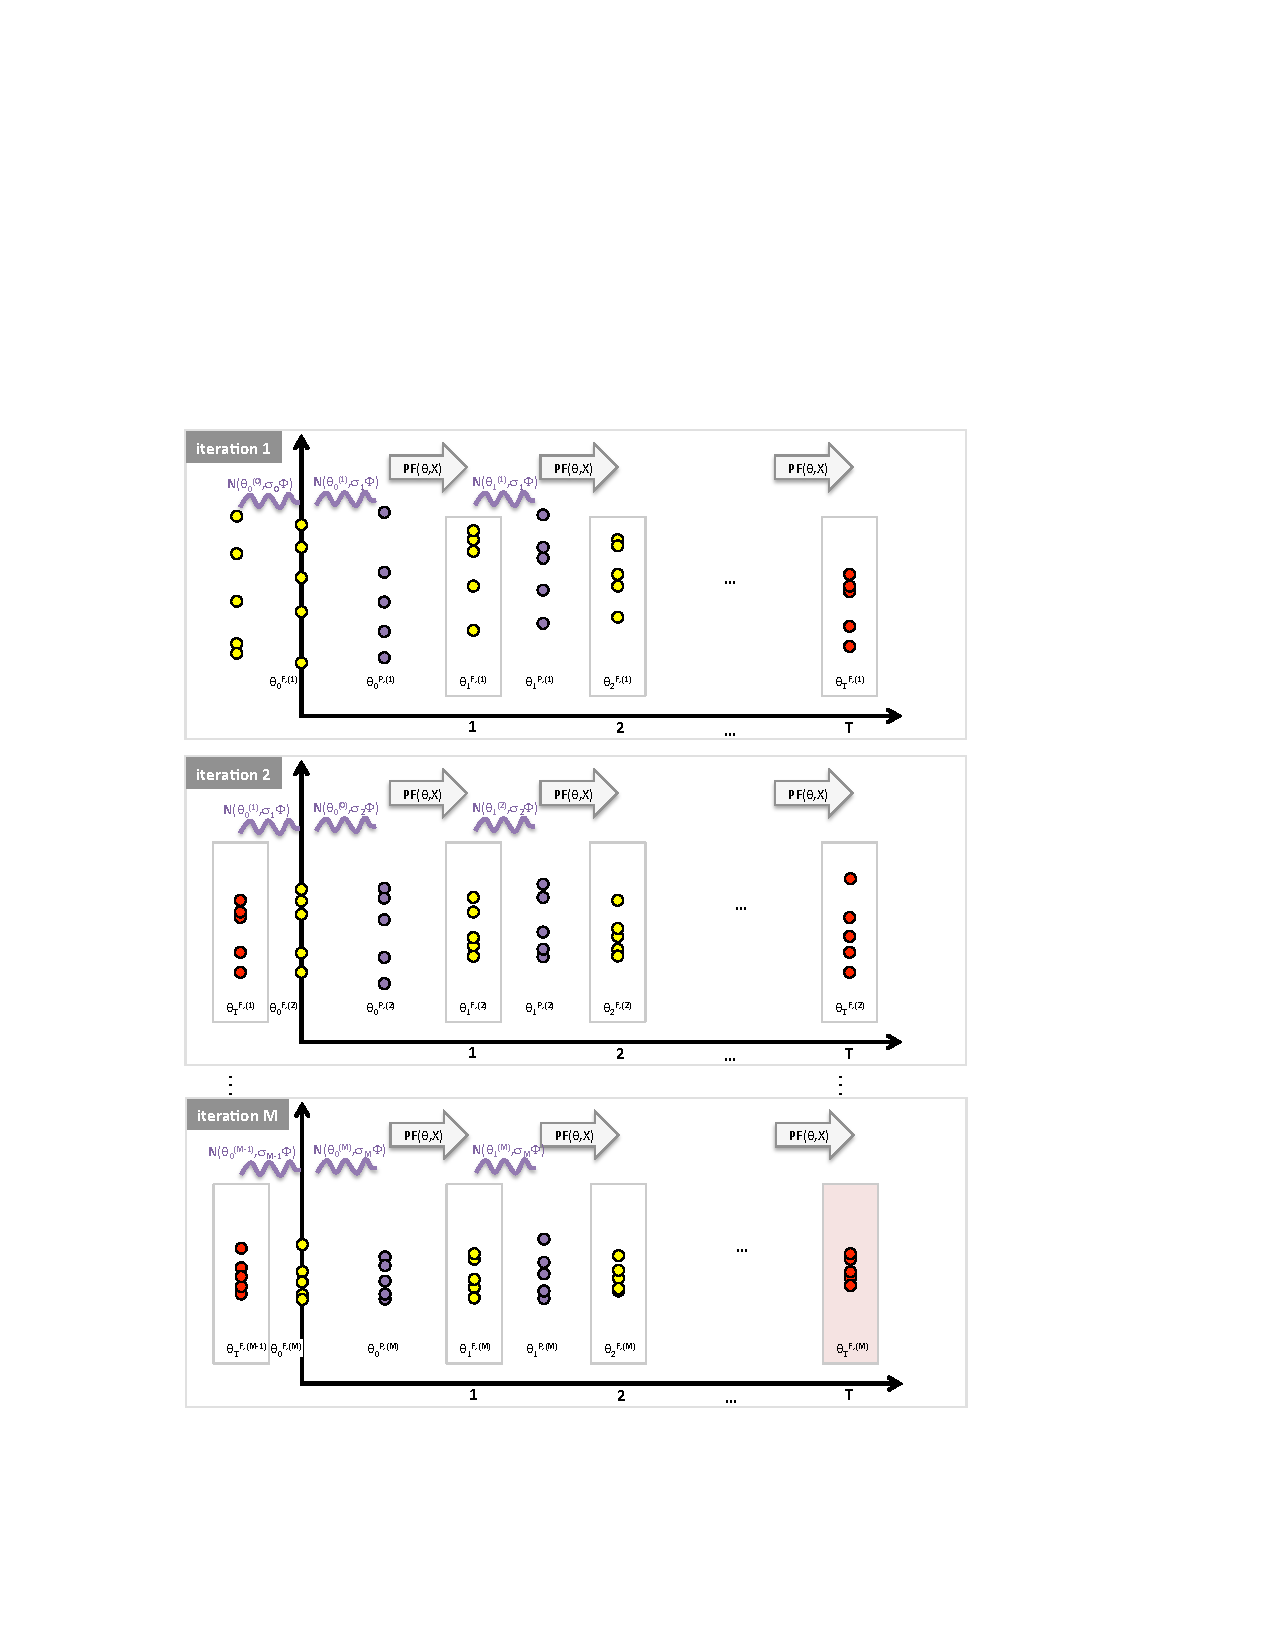
\includegraphics[width=\textwidth,height=0.7\textheight,keepaspectratio=true]{images/IF2-diagram}

		\end{column}
	\end{columns}

	\null
	\vspace{0.25\baselineskip}
	\centering
	\tiny
	Image source \cite{Doucet2001}

\end{frame}


%% 5. Fitting results
%%------------------------------------------
%%------------------------------------------


% Section title
\setbeamercolor{normal text}{fg=white, bg=Red}
\usebeamercolor[fg]{normal text}
\begin{frame}

	\vspace{2cm}
	\hspace{0.5cm} {\Huge Fitting Results }
	\begin{tikzpicture}[overlay]
	    \node[at=(current page.center), shift={(-4.5 cm, -4.7 cm)}, opacity=0.25] {
	    	\fontsize{200pt}{0pt}\selectfont
	        \color{white}{5}
	    };
	\end{tikzpicture}

\end{frame}

\setbeamercolor{normal text}{fg=Grey, bg=white}
\usebeamercolor[fg]{normal text}
\begin{frame}

	\begin{columns}
		\begin{column}{0.00001\textwidth}
		\null
		\end{column}

		\begin{column}{0.25\textwidth}

			\null
			\large
			IF2 \\
			\vspace{0.5\baselineskip}
			\footnotesize
			state estimates
			
		\end{column}
		\begin{column}{0.65\textwidth}

			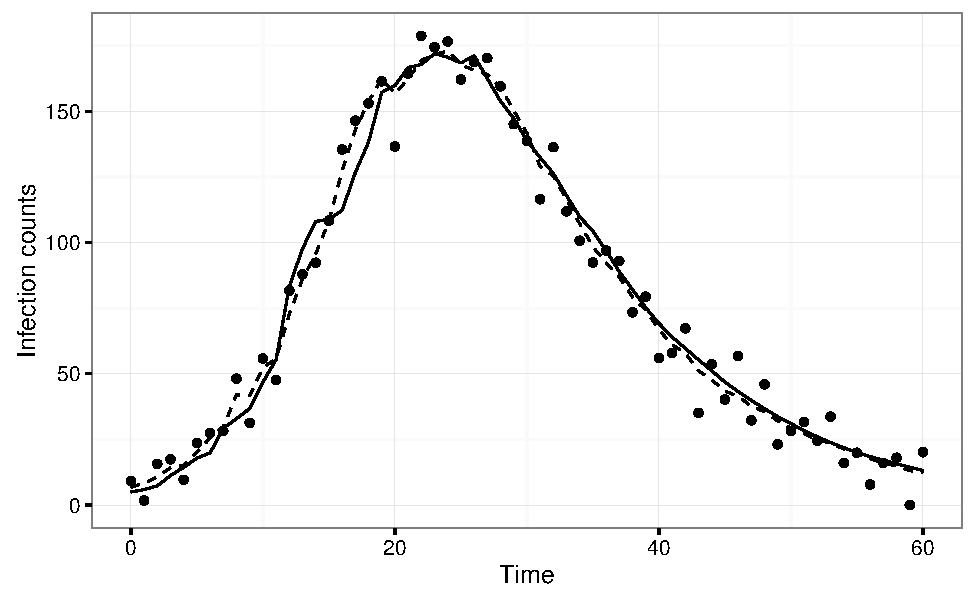
\includegraphics[width=\textwidth,height=0.45\textheight,keepaspectratio=true]{../../writing/SC1/images/if2state}

		\end{column}
	\end{columns}

	\textcolor{Grey50}{\rule{\textwidth}{0.4pt}} \\

	\begin{columns}
		\begin{column}{0.00001\textwidth}
		\null
		\end{column}

		\begin{column}{0.25\textwidth}

			\null
			\large
			HMC \\
			\vspace{0.5\baselineskip}
			\footnotesize
			state estimates
			
		\end{column}
		\begin{column}{0.65\textwidth}

			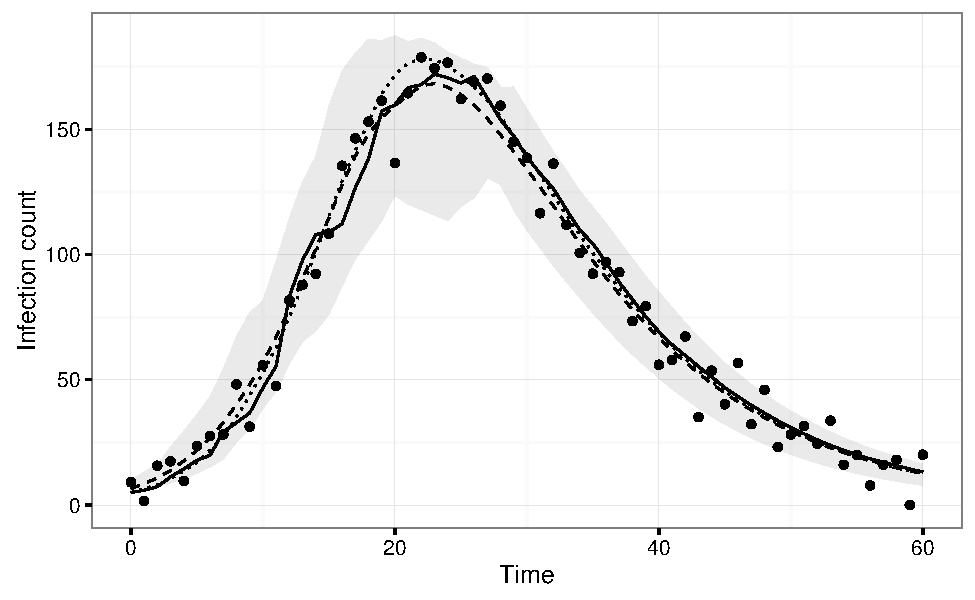
\includegraphics[width=\textwidth,height=0.45\textheight,keepaspectratio=true]{../../writing/SC1/images/hmcboot}

		\end{column}
	\end{columns}

	\vspace{0.5\baselineskip}
	\tiny
	\centering
	Dashed -- estimates $\quad\cdot\quad$ solid -- true $\quad\cdot\quad$ dots -- data $\quad\cdot\quad$ ribbon -- trajectories

\end{frame}


\setbeamercolor{normal text}{fg=Grey, bg=white}
\usebeamercolor[fg]{normal text}
\begin{frame}

	\begin{columns}
		\begin{column}{0.00001\textwidth}
		\null
		\end{column}

		\begin{column}{0.25\textwidth}

			\null
			\large
			IF2 \\
			\vspace{0.5\baselineskip}
			\footnotesize
			final particle swarm samples
			
		\end{column}
		\begin{column}{0.65\textwidth}

			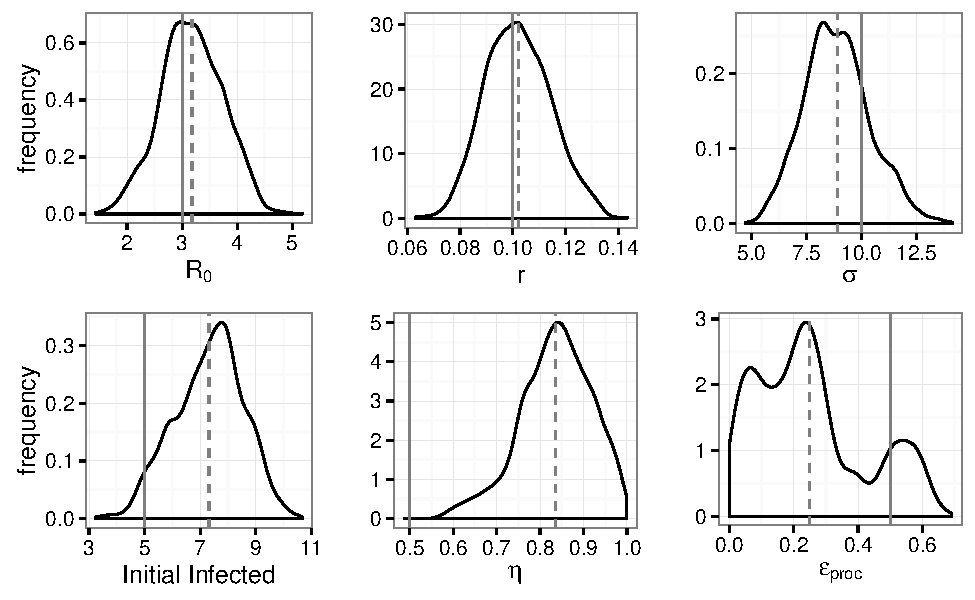
\includegraphics[width=\textwidth,height=0.45\textheight,keepaspectratio=true]{../../writing/SC1/images/if2kernels}

		\end{column}
	\end{columns}
	
	\textcolor{Grey50}{\rule{\textwidth}{0.4pt}} \\

	\begin{columns}
		\begin{column}{0.00001\textwidth}
		\null
		\end{column}

		\begin{column}{0.25\textwidth}

			\null
			\large
			HMC \\
			\vspace{0.5\baselineskip}
			\footnotesize
			posterior distribution estimates \\
			
		\end{column}
		\begin{column}{0.65\textwidth}

			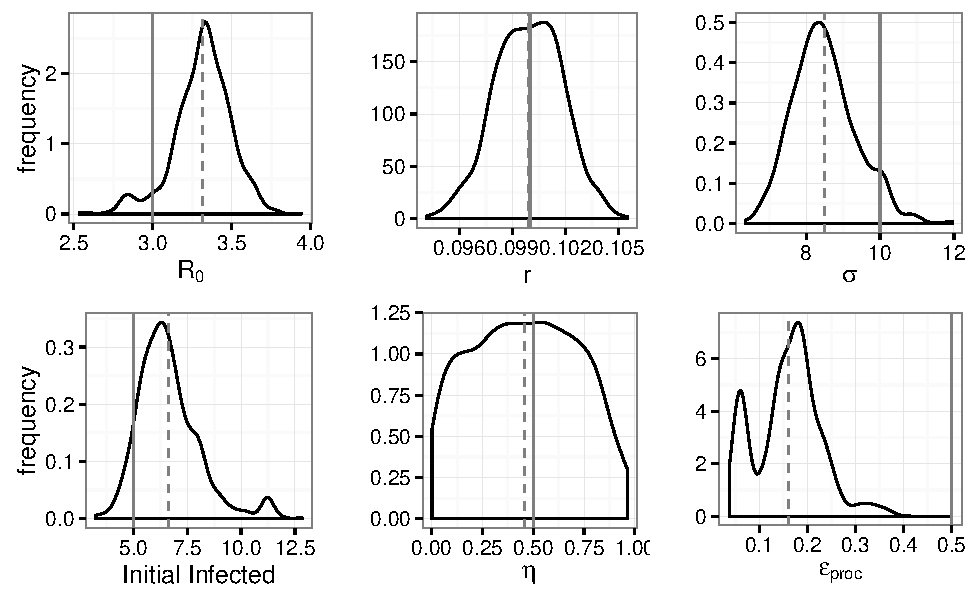
\includegraphics[width=\textwidth,height=0.45\textheight,keepaspectratio=true]{../../writing/SC1/images/hmckernels}

		\end{column}
	\end{columns}

	\tiny
	\vspace{0.5\baselineskip}
	\centering
	Dashed -- medians $\quad\cdot\quad$ solid -- true

\end{frame}


\setbeamercolor{normal text}{fg=Grey, bg=white}
\usebeamercolor[fg]{normal text}
\begin{frame}

	\null
	\large
	Mean parameter estimate distributions \\
	\vspace{\baselineskip}
	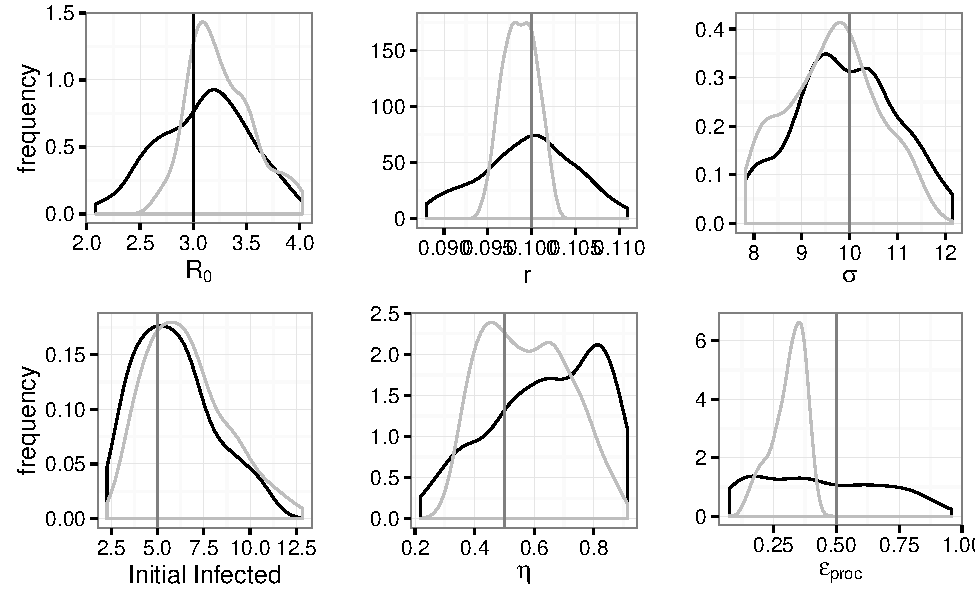
\includegraphics[width=\textwidth,height=\textheight,keepaspectratio=true]{../../writing/SC1/images/combined-multi} \\
	\centering
	\normalsize
	\textbf{IF2 \quad $\cdot$ \quad \textcolor{Grey50}{HMC}}

\end{frame}

\setbeamercolor{normal text}{fg=Grey, bg=white}
\usebeamercolor[fg]{normal text}
\begin{frame}

	\null
	\large
	Running times \\
	\vspace{\baselineskip}
	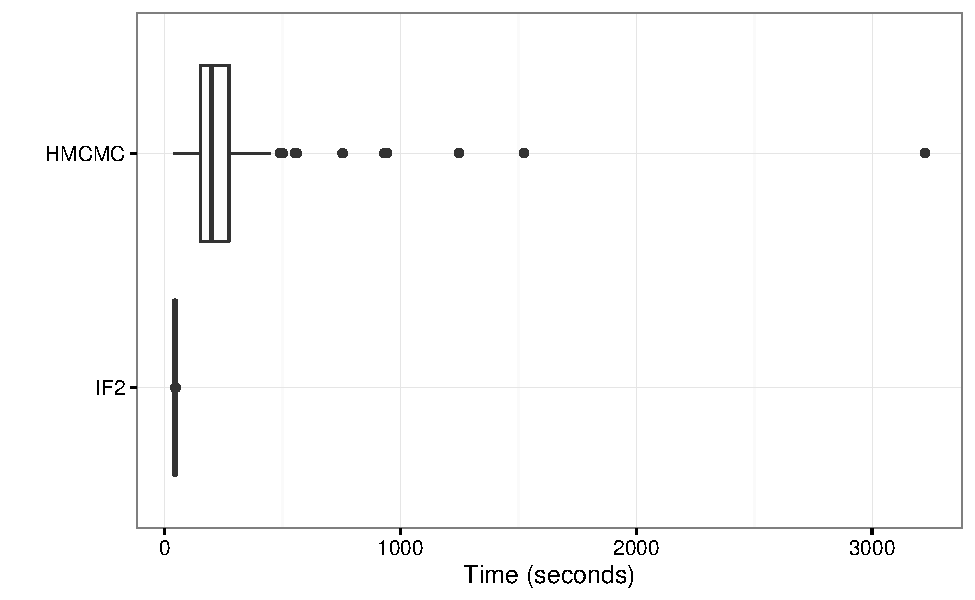
\includegraphics[width=\textwidth,height=\textheight,keepaspectratio=true]{../../writing/SC1/images/timeplot}

	\centering
	\vspace{0.5\baselineskip}
	\footnotesize
	IF2: 5.7x faster than HMC


\end{frame}

%%------------------------------------------
%%------------------------------------------


%% 5. Forecasting Frameworks
%% --------------------------------------------------------------------------------------
%% --------------------------------------------------------------------------------------

% Section title
\setbeamercolor{normal text}{fg=white, bg=Cyan}
\usebeamercolor[fg]{normal text}
\begin{frame}

	\vspace{2cm}
	\hspace{1cm} {\Huge Forecasting } \\
	\hspace{1cm} {\Huge Frameworks }
	\begin{tikzpicture}[overlay]
	    \node[at=(current page.center), shift={(-4 cm, -4.3 cm)}, opacity=0.25] {
	    	\fontsize{200pt}{0pt}\selectfont
	        \color{white}{6}
	    };
	\end{tikzpicture}

\end{frame}

\setbeamercolor{normal text}{fg=Grey, bg=white}
\usebeamercolor[fg]{normal text}
\begin{frame}

	\begin{columns}

		\begin{column}[t]{0.55\textwidth}

			\null
			\large
			IF2 \\
			\vspace{\baselineskip}

			\normalsize
			Parametric bootstrapping \\
			$+$ forward simulation
			\vspace{\baselineskip}
			
			\footnotesize
			\begin{itemize}
				\item Provides additional samples from posterior distribution
				\item Forward simulation using states point estimate, posterior samples
			\end{itemize}
			
		\end{column}
		\begin{column}[t]{0.45\textwidth}

			\null
			\large
			HMC \\
			\vspace{\baselineskip}
			\normalsize
			State reconstructions \\
			$+$ forward simulation
			\vspace{\baselineskip}
			
			\footnotesize
			\begin{itemize}
				\item Reconstruct states using latent process noise samples
				\item Simulate forward
			\end{itemize}

		\end{column}
	\end{columns}
	
\end{frame}

\setbeamercolor{normal text}{fg=Grey, bg=white}
\usebeamercolor[fg]{normal text}
\begin{frame}

	\begin{columns}
		\begin{column}{0.00001\textwidth}
		\null
		\end{column}

		\begin{column}{0.25\textwidth}

			\null
			\large
			IF2 \\
			\vspace{0.5\baselineskip}
			\footnotesize
			forecast
			
		\end{column}
		\begin{column}{0.65\textwidth}

			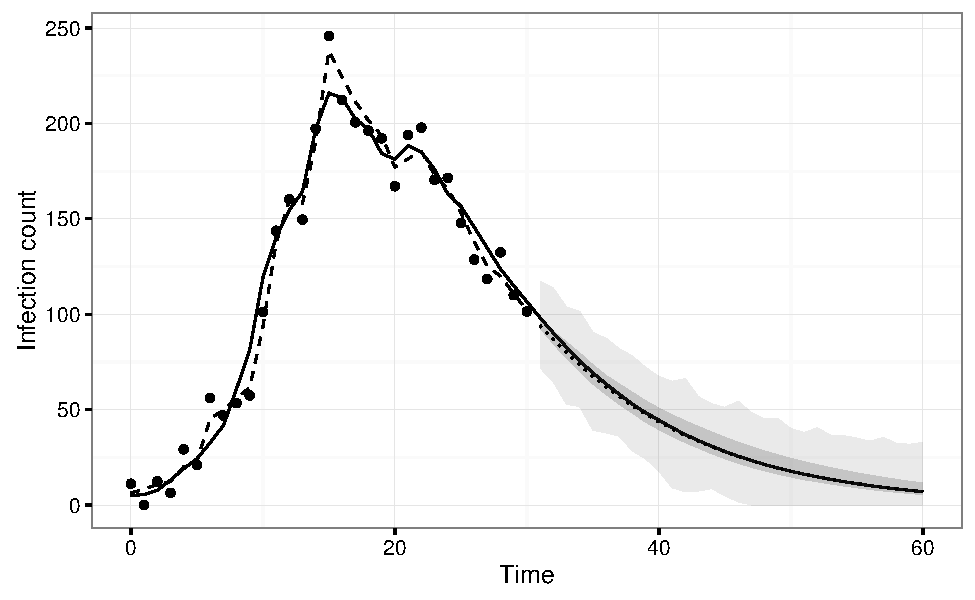
\includegraphics[width=\textwidth,height=0.45\textheight,keepaspectratio=true]{../../writing/SC2/images/if2combined}

		\end{column}
	\end{columns}
	
	\textcolor{Grey50}{\rule{\textwidth}{0.4pt}} \\

	\begin{columns}
		\begin{column}{0.00001\textwidth}
		\null
		\end{column}

		\begin{column}{0.25\textwidth}

			\null
			\large
			HMC \\
			\vspace{0.5\baselineskip}
			\footnotesize
			forecast
			
		\end{column}
		\begin{column}{0.65\textwidth}

			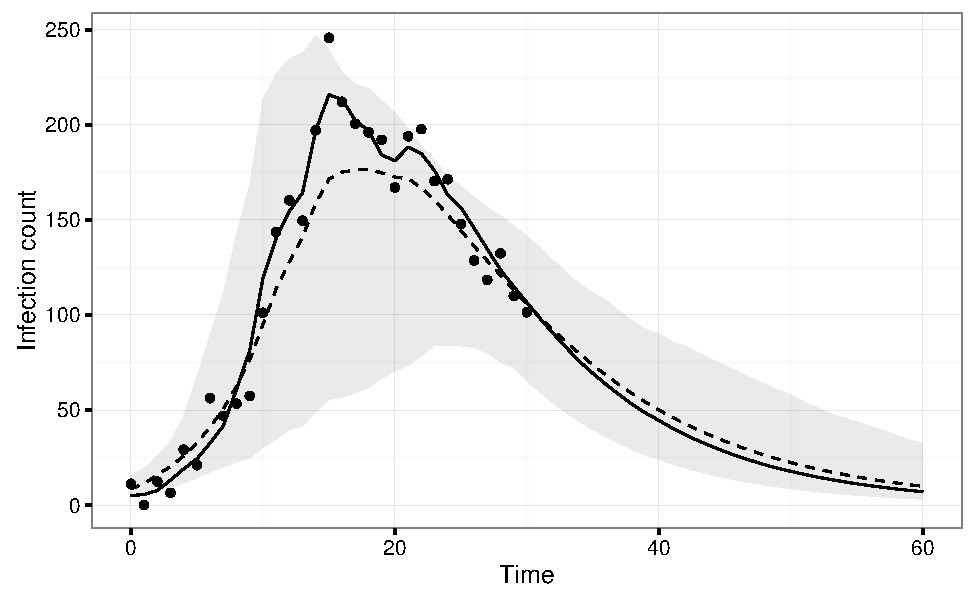
\includegraphics[width=\textwidth,height=0.45\textheight,keepaspectratio=true]{../../writing/SC2/images/hmcforecast}

		\end{column}
	\end{columns}

	\vspace{0.5\baselineskip}
	\tiny
	\centering
	Dotted/dashed -- mean $\quad\cdot\quad$ Dark ribbon - state $\quad\cdot\quad$ Light ribbon - observation

\end{frame}


\setbeamercolor{normal text}{fg=Grey, bg=white}
\usebeamercolor[fg]{normal text}
\begin{frame}

	\null
	\large
	Forecast accuracy comparison \\
	\vspace{\baselineskip}
	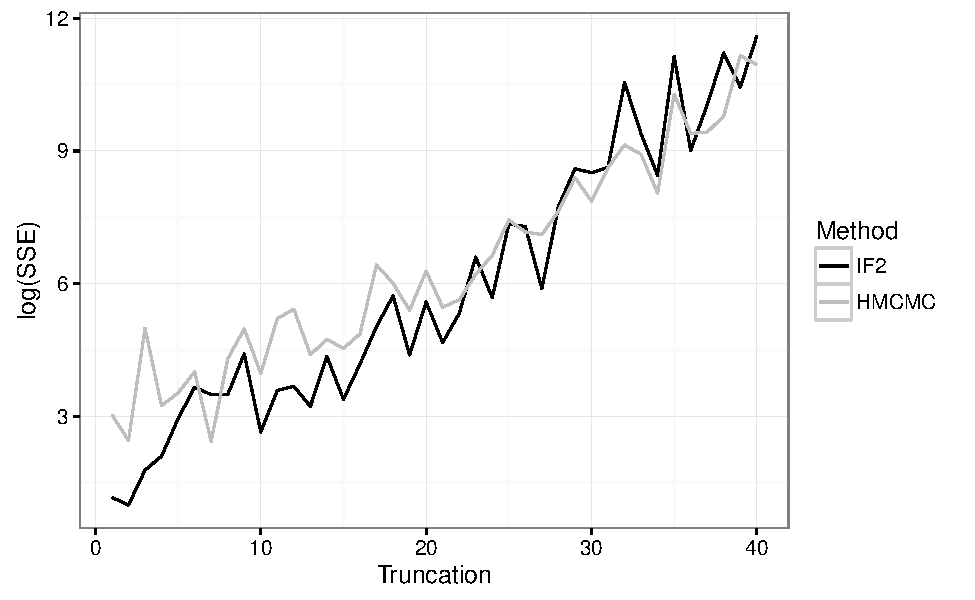
\includegraphics[width=\textwidth,height=\textheight,keepaspectratio=true]{../../writing/SC2/images/truncation}

\end{frame}


%% 6. S-maps and SIRS
%% --------------------------------------------------------------------------------------
%% --------------------------------------------------------------------------------------

% Section title
\setbeamercolor{normal text}{fg=white, bg=Indigo}
\usebeamercolor[fg]{normal text}
\begin{frame}

	\vspace{2cm}
	\hspace{-0.5cm} {\Huge S-maps \& } \\
	\hspace{-0.5cm} {\Huge Seasonal Outbreaks }
	\begin{tikzpicture}[overlay]
	    \node[at=(current page.center), shift={(-4.7 cm, -4.3 cm)}, opacity=0.25] {
	    	\fontsize{200pt}{0pt}\selectfont
	        \color{white}{7}
	    };
	\end{tikzpicture}

\end{frame}

% SIRS
\setbeamercolor{normal text}{fg=white, bg=Grey}
\setbeamercolor{footline}{parent=normal text}
\usebeamercolor[fg]{normal text}
\begin{frame}

	\null
	{\large \textcolor{Cyan}{Stochastic SIRS model}}
	\vfill

	\centering
	\begin{align*}
		\dfrac{dS}{dt} 	& = - \Gamma(t) \beta S I + \textcolor{Teal}{\alpha R}\\
		\dfrac{dI}{dt} 	& = \Gamma(t) \beta S I - \gamma I \\
		\dfrac{dR}{dt} 	& =  \gamma I - \textcolor{Teal}{\alpha R}
	\end{align*}
	\vspace{0.5\baselineskip}
	{\Large $+$}	\\
	\vspace{-0.5\baselineskip}
	\begin{align*}
		\Gamma (t) & = \exp \left[ 2 \left( \cos \left( \frac{2\pi}{365} t \right) \right) \right] \\
		& \\
		\beta_{t+1} & = \exp \left[ \beta_t + \eta \left( \bar{\beta} - \beta_t \right) + \mathcal{N}(0, \sigma_{\small\text{proc}}) \right]
	\end{align*}

\end{frame}

\setbeamercolor{normal text}{fg=Grey, bg=white}
\usebeamercolor[fg]{normal text}
\begin{frame}

	\null
	\large
	SIRS model simulation \\
	\vspace{\baselineskip}
	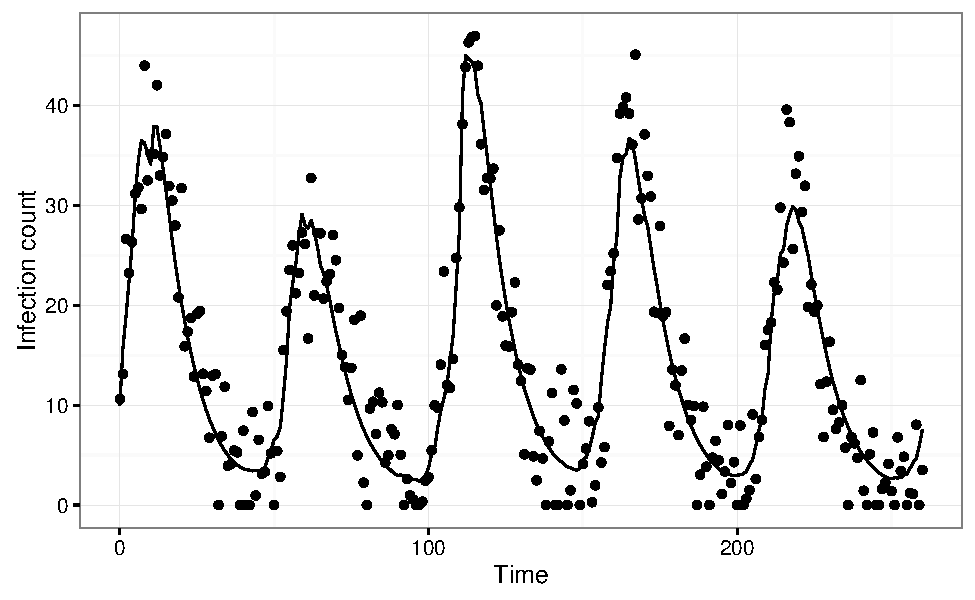
\includegraphics[width=\textwidth,height=\textheight,keepaspectratio=true]{../../writing/SIRS-SMAP/images/dataplot}

\end{frame}

\setbeamercolor{normal text}{fg=Grey, bg=white}
\usebeamercolor[fg]{normal text}
\begin{frame}

	\null
	\large
	S-map
	\vspace{\baselineskip}
	\footnotesize

	A little bit of history repeating

	\begin{itemize}
		\item Construct global weighted mapping of time-lagged vectors (the library) to future states
		\item Weightings are used to penalize poorly matching library vectors
	\end{itemize}

\end{frame}

\setbeamercolor{normal text}{fg=Grey, bg=white}
\usebeamercolor[fg]{normal text}
\begin{frame}

	\null
	\large
	S-map forecast \\
	\vspace{\baselineskip}
	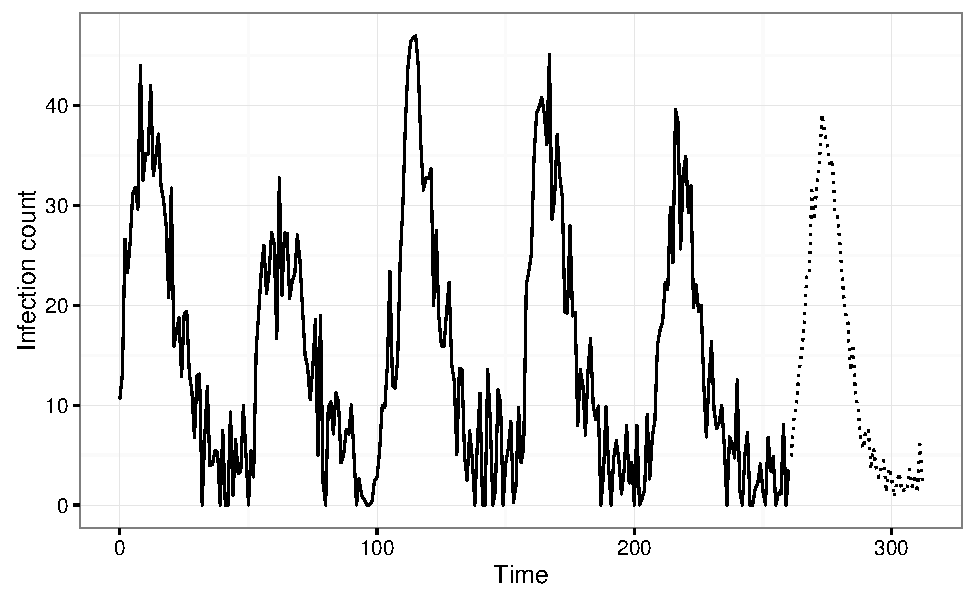
\includegraphics[width=\textwidth,height=\textheight,keepaspectratio=true]{../../writing/SIRS-SMAP/images/smap-project}

\end{frame}

\setbeamercolor{normal text}{fg=Grey, bg=white}
\usebeamercolor[fg]{normal text}
\begin{frame}

	\null
	\large
	SIRS model forecasting error \\
	\vspace{\baselineskip}
	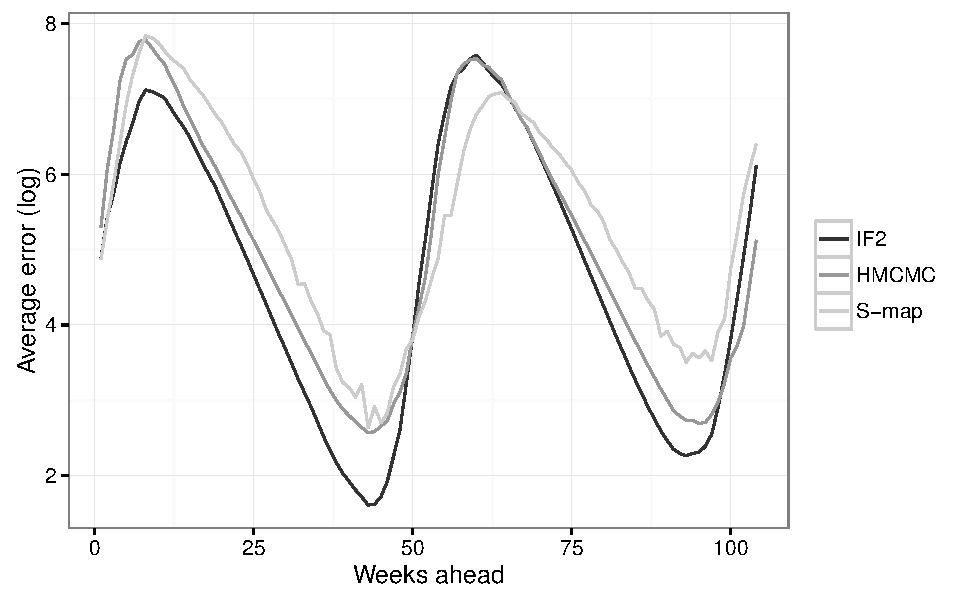
\includegraphics[width=\textwidth,height=\textheight,keepaspectratio=true]{../../writing/SIRS-SMAP/images/sseplot}

\end{frame}

\setbeamercolor{normal text}{fg=Grey, bg=white}
\usebeamercolor[fg]{normal text}
\begin{frame}

	\null
	\large
	SIRS model forecasting runtimes \\
	\vspace{\baselineskip}
	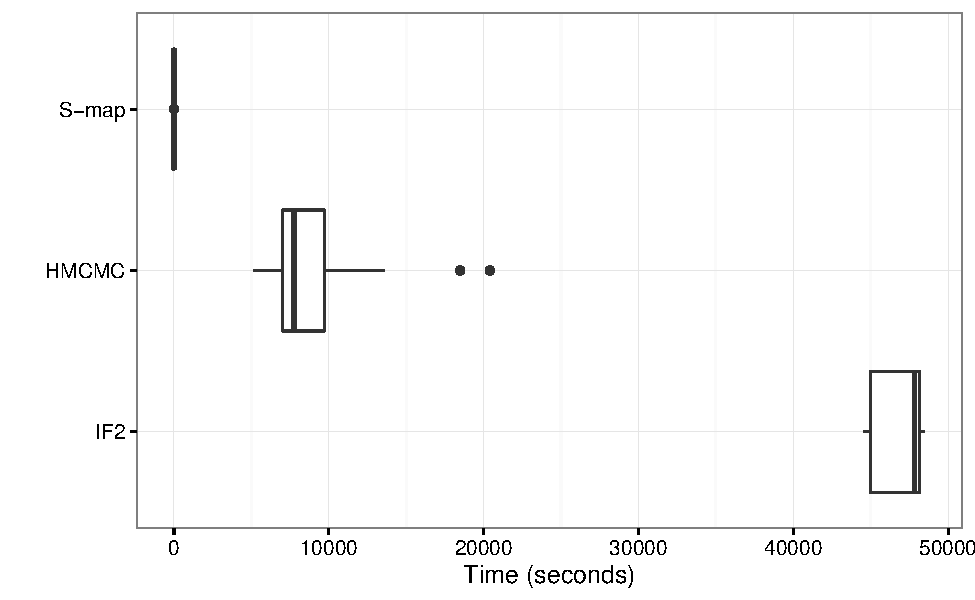
\includegraphics[width=\textwidth,height=\textheight,keepaspectratio=true]{../../writing/SIRS-SMAP/images/timeplot}
	\vfill

	\centering
	\vspace{0.5\baselineskip}
	\footnotesize
	S-map: 316,000x faster than IF2, 61,800x faster than HMC

\end{frame}


%% 7. Spatiotemporal
%% --------------------------------------------------------------------------------------
%% --------------------------------------------------------------------------------------

% Section title
\setbeamercolor{normal text}{fg=white, bg=BlueGrey}
\usebeamercolor[fg]{normal text}
\begin{frame}

	\vspace{2cm}
	\hspace{0cm} {\Huge Spatiotemporal } \\
	\vspace{0.1cm}
	\hspace{0cm} {\Huge Epidemics }
	\begin{tikzpicture}[overlay]
	    \node[at=(current page.center), shift={(-2 cm, -4.2 cm)}, opacity=0.25] {
	    	\fontsize{200pt}{0pt}\selectfont
	        \color{white}{8}
	    };
	\end{tikzpicture}

\end{frame}

\setbeamercolor{normal text}{fg=white, bg=Grey}
\usebeamercolor[fg]{normal text}
\begin{frame}

	\null
	{\large \textcolor{Cyan}{Stochastic Spatial SIR model}}
	\vfill

	\centering
	\begin{align*}
		\dfrac{dS_i}{dt} 	& = - \left(1-\textcolor{Teal}{\phi \frac{M}{M+1}} \right) \beta_i S_i I_i - \textcolor{Teal}{ \frac{\phi}{M+1} } S_i \textcolor{PaleYellow}{\sum_{j = 1}^{M} \beta_{ij}{I_j}} \\
		\dfrac{dI_i}{dt} 	& = \left(1-\textcolor{Teal}{\phi \frac{M}{M+1}} \right) \beta_i S_i I_i + \textcolor{Teal}{ \frac{\phi}{M+1} } S_i \textcolor{PaleYellow}{\sum_{j = 1}^{M} \beta_{ij}{I_j}} - \gamma I_i\\
		\dfrac{dR_i}{dt} 	& = \gamma I_i
	\end{align*}
	\vspace{\baselineskip}
	{\Large $+$} \\
	$\beta_{i,t+1} = \exp \left[ \beta_{i,t} + \eta \left( \bar{\beta} - \beta_{i,t} \right) + \mathcal{N}(0, \sigma_{\small\text{proc}}) \right]$

\end{frame}

\setbeamercolor{normal text}{fg=Grey, bg=white}
\usebeamercolor[fg]{normal text}
\begin{frame}

	\null
	\vfill
	Stochastic spatial SIR model simulation (ring topology) \\
	\vspace{\baselineskip}
	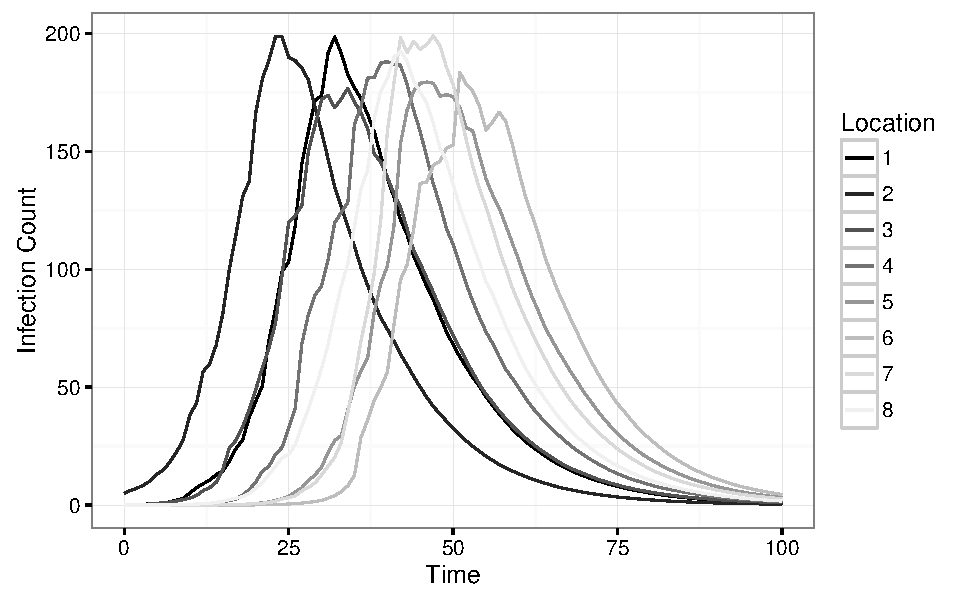
\includegraphics[width=\textwidth,height=\textheight,keepaspectratio=true]{../../writing/SPATIAL/images/dataplot}
	\vfill

\end{frame}

\setbeamercolor{normal text}{fg=Grey, bg=white}
\usebeamercolor[fg]{normal text}
\begin{frame}

	Dewdrop Regression
	\vspace{\baselineskip}

	\begin{itemize}
		\item ``Stitching'' together multiple short time series into single library
		\item Requires scaling
	\end{itemize}

\end{frame}

\setbeamercolor{normal text}{fg=Grey, bg=white}
\usebeamercolor[fg]{normal text}
\begin{frame}

	\null
	\large
	Spatial SIR model forecasting error \\
	\vspace{\baselineskip}
	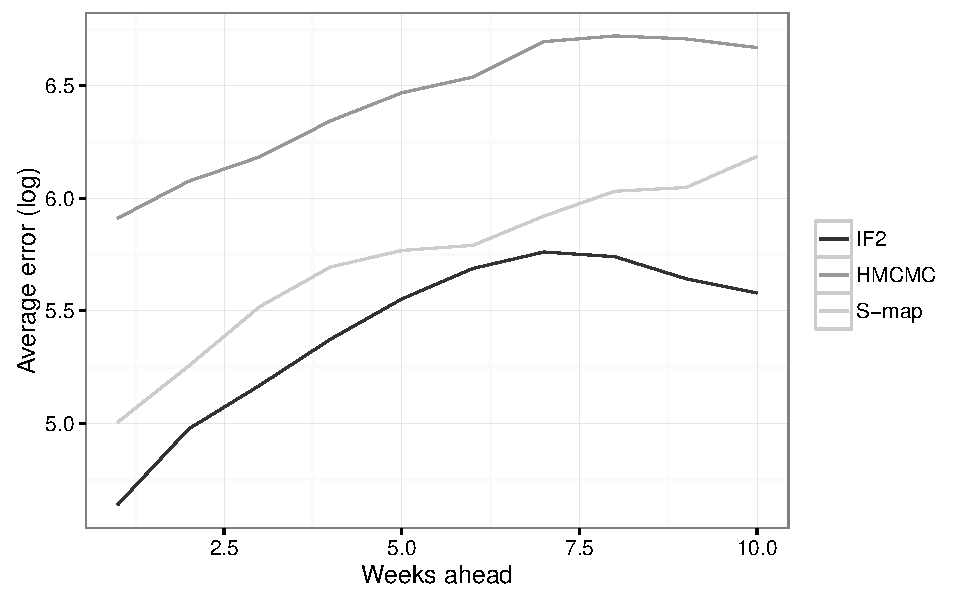
\includegraphics[width=\textwidth,height=\textheight,keepaspectratio=true]{../../writing/SPATIAL/images/sseplot}

\end{frame}

\setbeamercolor{normal text}{fg=Grey, bg=white}
\usebeamercolor[fg]{normal text}
\begin{frame}

	\null
	\large
	Spatial SIR model forecasting runtimes \\
	\vspace{\baselineskip}
	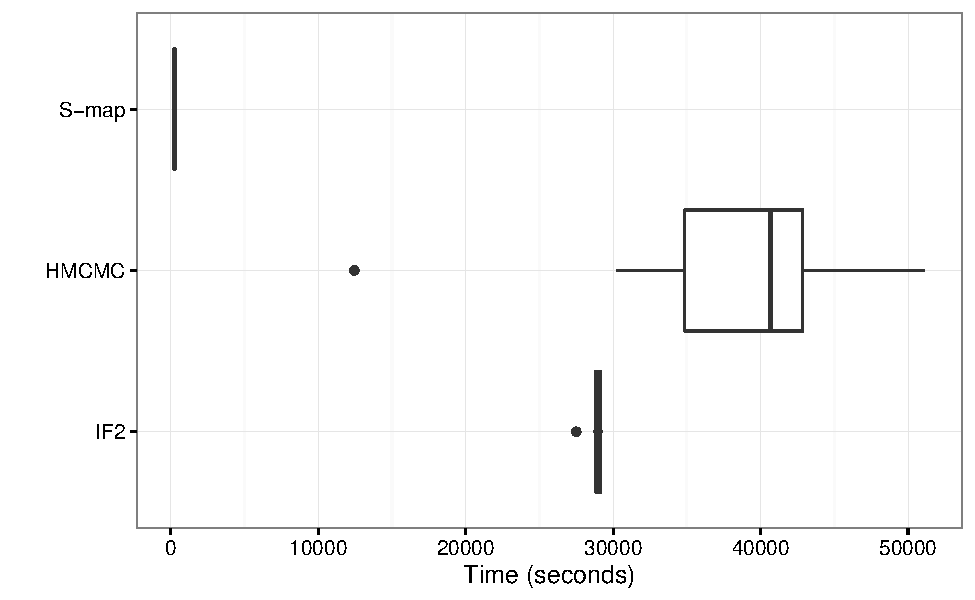
\includegraphics[width=\textwidth,height=\textheight,keepaspectratio=true]{../../writing/SPATIAL/images/timeplot}

	\centering
	\vspace{0.5\baselineskip}
	\footnotesize
	S-map: 116x faster than IF2, 156x faster than HMC

\end{frame}

%% 8. Parallelism and Future Directions
%% --------------------------------------------------------------------------------------
%% --------------------------------------------------------------------------------------

% Section title
\setbeamercolor{normal text}{fg=white, bg=DeepOrange}
\usebeamercolor[fg]{normal text}
\begin{frame}

	\vspace{2cm}
	\hspace{0cm} {\Huge Parallelism \& } \\
	\vspace{0.3cm}
	\hspace{0cm} {\Huge Future Directions }
	\begin{tikzpicture}[overlay]
	    \node[at=(current page.center), shift={(-4.7 cm, -4.3 cm)}, opacity=0.25] {
	    	\fontsize{200pt}{0pt}\selectfont
	        \color{white}{9}
	    };
	\end{tikzpicture}

\end{frame}

\setbeamercolor{normal text}{fg=Grey, bg=white}
\usebeamercolor[fg]{normal text}
\begin{frame}

	Conclusions
	\vspace{\baselineskip}

	\begin{itemize}
		\item IF2 produces superior forecasts in all scenarios
		\item S-mapping runs orders of magnitude faster than other methods
	\end{itemize}

\end{frame}

\setbeamercolor{normal text}{fg=Grey, bg=white}
\usebeamercolor[fg]{normal text}
\begin{frame}

	More than Moore
	\vspace{\baselineskip}

	\begin{itemize}
		\item Moore's Law is ceasing to hold
		\item Focus now on distributed computing
		\item MCMC-based methods are resistant to parallelization
		\begin{itemize}
		 	\item Chain construction \textit{requires} iterative dependence
		\end{itemize} 
		\item IF2 exhibits high parallel potential
		\begin{itemize}
			\item Preliminary CUDA (GPU-accelerated) implementation - \texttt{cuIF2}
		\end{itemize}
	\end{itemize}

\end{frame}

\setbeamercolor{normal text}{fg=Grey, bg=white}
\usebeamercolor[fg]{normal text}
\begin{frame}

	\null
	\large
	Spatial SIR model fitting times \\
	\vspace{\baselineskip}
	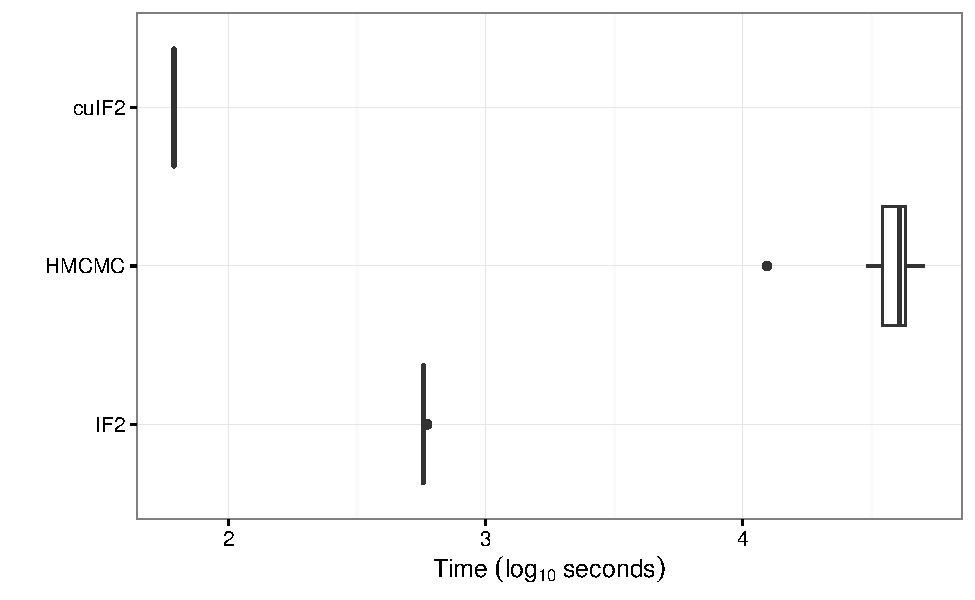
\includegraphics[width=\textwidth,height=\textheight,keepaspectratio=true]{../../writing/SPATIAL/images/timeplot2}

	\centering
	\vspace{0.5\baselineskip}
	\footnotesize
	\texttt{cuIF2}: 9.33x faster than IF2, 617x faster than HMC

\end{frame}


\setbeamercolor{normal text}{fg=white, bg=Grey}
\usebeamercolor[fg]{normal text}
\begin{frame}
	
	\null
	\vspace{\baselineskip}
	\centering
	\huge
	Questions

\end{frame}

\setbeamercolor{normal text}{fg=Grey, bg=white}
\setbeamercolor{bibliography item}{parent=normal text}
\usebeamercolor[fg]{normal text}
\begin{frame}
	\nocite{*}
	\bibliographystyle{abbrv}
	\bibliography{defence-refs}
\end{frame}


\setbeamercolor{normal text}{fg=Grey, bg=white}
\usebeamercolor[fg]{normal text}
\begin{frame}

	\null
	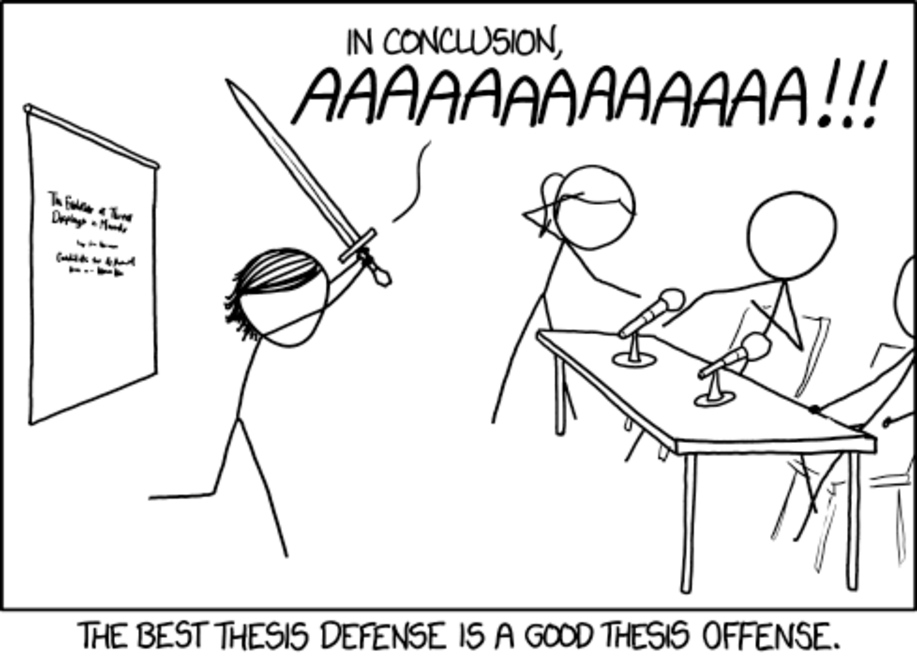
\includegraphics[width=\textwidth,height=\textheight,keepaspectratio=true]{images/thesis_defense}

\end{frame}


\end{document}